\chapter{Технологический раздел}
\vspace{-0.5cm}	\hspace{0.6cm}В данном разделе будут рассмотрены требования к разрабатываемому программному обеспечиванию, средства, использованные в процессе разработки для реализации поставленных задач, а также представлены листинги кода программы. Будет описаны основные функции интерфейса программы и примеры работы программы (результат рендера).

\section{Требования к программному обеспечению}
\hspace{0.6cm}Программное обеспечение должно реализовывать поставленную на курсовой проект задачу. В программном модуле должен присутствовать интерфейс для взаимодействия с объектом. Программа не должна аварийно завершаться, сильно нагружать процессор, а также не должна задействовать большой объем оперативной памяти.

\section{Средства реализации}
\hspace{0.6cm}Для реализации программы был использован язык программирования С++ (стандарт GNU++11\cite{web:cpp}). С++ имеет достаточный функционал в стандартных библиотеках, поддерживает многопоточность выполнения программы и является высокопроизводительным языком, что важно при реализации задача высокой нагрузки, таких как рендеринг.

\vspace{0.2cm}Проект выполнен в среде разработки QtCreator с использованием сопутствующей графической оболочки QtGraphics\cite{web:qt}. Данная оболочка предоставляет удобный функционал отрисовки графических объектов по пикселям, а также возможность создания удобного интерфейса для взаимодействия с пользователем. Платформа включает в себя архитектуру распространения событий, которая позволяет использовать возможности взаимодействия элементов на сцене.

\section{Сборка и запуск проекта}
\hspace{0.6cm}Для сборки проекта используется компилятор g++ и система сборки qmake, поставляемая Qt\cite{web:qt}. Система сборки qmake автоматически генерирует файлы сборки make, основываясь на информации в файлах проекта. Для корректной сборки приложения необходимы стандартные библиотеки языка C++ (включая библиотеки пространства имён std) и библиотеки QtGraphics.

\section{Реализация структур и алгоритмов}
\hspace{0.6cm}На основе схем, приведённых в конструкторском разделе, в соответствии с указанными требованиями к реализации было разработано программное обеспечение, содержащее реализации выбранных алгоритмов. В данном подразделе приведены листинги \ref{list:vertex}-\ref{list:update} реализаций структур данных и алгоритма.

\begin{lstlisting}[caption=Класс <<вершина>> Vertex, label=list:vertex]
class Vertex
{
public:
	Vertex() : _x(0), _y(0), _z(0) {}
	Vertex(double x, double y, double z) : _x(x), _y(y), _z(z) {}
	Vertex(const Vertex &vertex);
	Vertex(Vertex &&vertex);
	
	Vertex& operator=(const Vertex &vertex);
	Vertex& operator=(Vertex &&vertex);
	
	double x();
	double y();
	double z();
	
	void set_x(double x);
	void set_y(double y);
	void set_z(double z);
	void set(double x, double y, double z);
	
	void shift(double dx, double dy, double dz);
	void scale(double kx, double ky, double kz, Vertex pc = Vertex(0, 0, 0));
	void rotate_x(double angle, Vertex pc = Vertex(0, 0, 0));
	void rotate_y(double angle, Vertex pc = Vertex(0, 0, 0));
	void rotate_z(double angle, Vertex pc = Vertex(0, 0, 0));
	
	void shift(std::vector<double> d);
	void scale(std::vector<double> k, Vertex pc = Vertex(0, 0, 0));
	void rotate(std::vector<double> a, Vertex pc = Vertex(0, 0, 0));

private:
	double _x, _y, _z;
};

double distance(Vertex &p1, Vertex &p2);
\end{lstlisting}

\begin{lstlisting}[caption=Класс <<грань>> Trinangle, label=list:triangle]
class Triangle
{
public:
	Triangle(size_t i1, size_t i2, size_t i3, QColor c=QColor(255, 0, 0));
	Triangle(const Triangle &tr);
	Triangle(Triangle &&tr);
	
	Triangle& operator=(const Triangle &tr);
	Triangle& operator=(Triangle &&tr);
	
	size_t get_vertex(size_t index);
	void set_vertex(size_t index, size_t value);
	
	std::vector<Vertex> get_vertices(std::vector<Vertex>& vertices);
	std::vector<MathVector> get_normals(std::vector<MathVector>& normals);
	
	QColor get_color() const;
	void set_color(QColor c);

private:
	size_t vertex_indexes[3];
	QColor colour;
};
\end{lstlisting}

\begin{lstlisting}[caption=Класс <<модель>> Model, label=list:model]
class Model : public VisibleObject
{
public:
	Model() {}
	Model(const Model &model);
	Model(Model &&model);
	~Model() = default;
	
	Model& operator=(const Model &model);
	Model& operator=(Model &&model);
	
	std::vector<Vertex>& get_vertices();
	std::vector<Triangle>& get_triangles();
	
	void shift(double dx, double dy, double dz);
	void scale(double kx, double ky, double kz, Vertex pc=Vertex(0, 0, 0));
	void rotate(double ax, double ay, double az, Vertex pc=Vertex(0, 0, 0));
	
	void shift(std::vector<double> d);
	void scale(std::vector<double> k, Vertex pc = Vertex(0, 0, 0));
	void rotate(std::vector<double> a, Vertex pc = Vertex(0, 0, 0));
	
	std::vector<MathVector> get_normals();

private:
	std::vector<Vertex> vertices;
	std::vector<Triangle> triangles;
};
\end{lstlisting}

\begin{lstlisting}[caption=Класс <<узел>> Node, label=list:mwidget]
class Node
{
public:
	Node(const Vertex& v, size_t index, double mass, double friction);
	~Node() = default;
	
	Vertex start_pos;
	double mass;
	double inv_mass;
	double friction;
	MathVector f;
	MathVector v;
	size_t vertex_index;
	std::shared_ptr<Vertex> vertex;
};
\end{lstlisting}

\begin{lstlisting}[caption=Класс <<ребро>> Edge, label=list:edge]
class Edge
{
public:
	Edge(const Node &node1, const Node &node2, double spring_rate,
	double friction);
	~Edge() = default;
	
	size_t v1;
	size_t v2;
	double len_rest;
	double len_cur;
	double spring_rate;
	double friction;
};
\end{lstlisting}

\begin{lstlisting}[caption=Класс <<флаг>> Flag, label=list:work_render]
class Flag
{
public:
	Flag(Vertex topleft, double w, double h, QColor colour);
	~Flag() = default;
	
	std::shared_ptr<Model> get_model();
	
	void set_mass(double mass);
	void set_friction(double friction);
	void set_spring(double spring_rate);
	
	void reset();
	void update(MathVector wind_vector, int msec);
	void update_thread(MathVector wind_vector, int msec);

private:
	Model model;
	std::vector<Node> nodes;
	std::vector<Edge> edges;
	
	Model start_model;
	std::vector<Node> start_nodes;
	std::vector<Edge> start_edges;
	
	void update_nodes_init(size_t start, size_t end);
	void update_wind_tr(MathVector& wv, size_t start, size_t end,
	std::vector<Vertex>& v, std::vector<Triangle>& tr);
	void update_edges(size_t start, size_t end, std::vector<Vertex>& v);
	void update_nodes(int msec, size_t start, size_t end,
	std::vector<Vertex>& v);
};
\end{lstlisting}

\begin{lstlisting}[caption=Функции аффинных преобразований, label=list:affin]
void Vertex::shift(double dx, double dy, double dz)
{
	_x += dx;
	_y += dy;
	_z += dz;
}

void Vertex::scale(double kx, double ky, double kz, Vertex pc)
{
	double px = pc.x(), py = pc.y(), pz = pc.y();
	_x = px + (_x - px) * kx;
	_y = py + (_y - py) * ky;
	_z = pz + (_z - pz) * kz;
}

void Vertex::rotate_x(double angle, Vertex pc)
{
	double py = pc.y(), pz = pc.z();
	double dy = _y - py, dz = _z - pz;
	_y = py + dy * cos(angle) - dz * sin(angle);
	_z = pz + dy * sin(angle) + dz * cos(angle);
}

void Vertex::rotate_y(double angle, Vertex pc)
{
	double pz = pc.z(), px = pc.x();
	double dz = _z - pz, dx = _x - px;
	_z = pz + dz * cos(angle) - dx * sin(angle);
	_x = px + dz * sin(angle) + dx * cos(angle);
}

void Vertex::rotate_z(double angle, Vertex pc)
{
	double px = pc.x(), py = pc.y();
	double dx = _x - px, dy = _y - py;
	_x = px + dx * cos(angle) - dy * sin(angle);
	_y = py - dx * sin(angle) + dy * cos(angle);
}
\end{lstlisting}

\begin{lstlisting}[caption=Функция отрисовки грани, label=list:draw_triangle]
void ModelDrawer::draw_triangle(std::vector<Vertex> v,
								std::vector<MathVector> n,
								MathVector l, QColor colour, bool outline)
{
	if (v[0].y() == v[1].y() && v[0].y() == v[2].y())
		return;
	
	double intens[3];
	for (int i = 0; i < 3; i++)
		intens[i] = abs(n[i] & l);
	
	if (v[0].y() > v[1].y())
	{
		std::swap(v[0], v[1]);
		std::swap(intens[0], intens[1]);
	}
	
	if (v[0].y() > v[2].y())
	{
		std::swap(v[0], v[2]);
		std::swap(intens[0], intens[2]);
	}
	
	if (v[1].y() > v[2].y())
	{
		std::swap(v[1], v[2]);
		std::swap(intens[1], intens[2]);
	}
	
	Vertex v_zero(0, 0, 0);
	MathVector vec[] = { MathVector(v_zero, v[0]),
	MathVector(v_zero, v[1]),
	MathVector(v_zero, v[2]) };
	
	double dy_0_2 = v[2].y() - v[0].y();
	double dy_0_1 = v[1].y() - v[0].y();
	double dy_1_2 = v[2].y() - v[1].y();
	
	double ia_0 = intens[0] / dy_0_1;
	double ia_1 = intens[1] / dy_0_1;
	double ib_0 = intens[0] / dy_0_2;
	double ib_2 = intens[2] / dy_0_2;
	
	for (int i = 0; i < dy_0_2; i++)
	{
		bool second_half = (i > dy_0_1) || (v[1].y() == v[0].y());
		double seg_height = second_half ? dy_1_2 : dy_0_1;
		
		double alpha = i / dy_0_2;
		double beta = 1.0;
		if (second_half)
			beta = (i - dy_0_1) / seg_height;
		else
			beta = i / seg_height;
		
		MathVector A = vec[0] + alpha * (vec[2] - vec[0]);
		MathVector B;
		if (second_half)
			B = vec[1] + beta * (vec[2] - vec[1]);
		else
			B = vec[0] + beta * (vec[1] - vec[0]);
		
		if (A.x() > B.x())
			std::swap(A, B);
		
		double dx = B.x() - A.x();
		double ddx = (dx == 0) ? 0.0 : 1 / dx;
		double ia = (dx == 0) ? 0.0 : (ia_0 * (v[1].y() - A.y()) +
		ia_1 * (A.y() - v[0].y())) / dx;
		double ib = (dx == 0) ? 0.0 : (ib_0 * (v[2].y() - B.y()) +
		ib_2 * (B.y() - v[0].y())) / dx;
		
		for (int x = 0; x <= dx; x++)
		{
			MathVector P = A + x * ddx * (B - A);
			double intens_p = ia * (B.x() - P.x()) + ib * (P.x() - A.x());
			
			int idx = round(P.x());
			int idy = round(P.y());
			
			if (idx >= 0 && idx < IMG_SIZE && idy >= 0 && idy < IMG_SIZE &&
				z_buf[idx][idy] < P.z())
			{
				z_buf[idx][idy] = int(round(P.z()));
				
				int r = round(colour.red() * abs(intens_p));
				int g = round(colour.green() * abs(intens_p));
				int b = round(colour.blue() * abs(intens_p));
				
				if (r > 255)
					r = 255;
				if (g > 255)
					g = 255;
				if (b > 255)
					b = 255;
				
				c_buf[idx][idy] = QColor(r, g, b);
			}
		}
	}
	
	if (outline)
	{
		colour = colour.darker(120);
		draw_edge(v[0], v[1], colour);
		draw_edge(v[1], v[2], colour);
		draw_edge(v[0], v[2], colour);
	}
}
\end{lstlisting}

\begin{lstlisting}[caption=Функция отрисовки сцены, label=list:draw_model]
void ModelDrawer::draw_scene(std::vector<Model> models, Camera& cam)
{
	QImage &img = canvas->get_image();
	QColor bg_color(180, 240, 240);
	img.fill(bg_color);
	
	if (models.size() == 0)
		return;
	
	for (int i = 0; i < IMG_SIZE; i++)
	{
		for (int j = 0; j < IMG_SIZE; j++)
		{
			z_buf[i][j] = -INT_MAX;
			c_buf[i][j] = bg_color;
		}
	}
	
	Vertex light_pos = light;
	
	light_pos.shift(cam.get_shift_params());
	light_pos.scale(cam.get_scale_params(), cam.get_center());
	light_pos.rotate(cam.get_rotate_params(), cam.get_center());
	
	light_pos.shift(canv_shift);
	light_pos.rotate(canv_rotate, canv_center);
	
	std::vector<double>& params = cam.get_rotate_params();
	
	Vertex v0(0, 0, 0);
	
	v0.shift(cam.get_shift_params());
	v0.scale(cam.get_scale_params(), cam.get_center());
	v0.rotate(cam.get_rotate_params(), cam.get_center());
	
	v0.shift(canv_shift);
	v0.rotate(canv_rotate, canv_center);
	
	MathVector l(v0, light_pos);
	l.normalize();
	
	for (auto model : models)
	{
		std::vector<Vertex>& vertices = model.get_vertices();
		std::vector<Triangle>& triangles = model.get_triangles();
		
		for (size_t i = 0; i < vertices.size(); i++)
		{
			vertices[i].shift(canv_shift);
			vertices[i].rotate(canv_rotate, canv_center);
		}
		
		std::vector<MathVector> normals = model.get_normals();
		
		for (auto tr : triangles)
		{
			std::vector<Vertex> v = tr.get_vertices(vertices);
			std::vector<MathVector> n = tr.get_normals(normals);
			draw_triangle(v, n, l, tr.get_color());
		}
	}
	
	size_t di = IMG_SIZE / 4, i = 0;
	
	std::vector<std::thread> threads;
	for (size_t k = 0; k < 4; k++, i += di)
		threads.push_back(std::thread(ModelDrawer::fill_buffer,
							  this, std::ref(img), i, i + di));
	
	for (size_t k = 0; k < 4; k++)
		threads[k].join();
	
	canvas->repaint();
}
\end{lstlisting}

\begin{lstlisting}[caption=Функция обновления положения точки флага, label=list:update]
void Flag::update_thread(MathVector wv, int msec)
{
	std::vector<Vertex>& v = model.get_vertices();
	std::vector<Triangle>& tr = model.get_triangles();
	
	size_t dn = nodes.size() / 4;
	std::vector<std::thread> threads_init;
	for (size_t k = 0, i = 0; k < 4; k++, i += dn)
		threads_init.push_back(std::thread(Flag::update_nodes_init,
							   this, i,
							   (k == 3 ? nodes.size() : i + dn)));
	for (size_t k = 0; k < 4; k++)
		threads_init[k].join();
	
	size_t dt = tr.size() / 4;
	std::vector<std::thread> threads_tr;
	for (size_t k = 0, i = 0; k < 4; k++, i += dt)
		threads_tr.push_back(std::thread(Flag::update_wind_tr,
									 this, std::ref(wv), i,
									 (k == 3 ? tr.size() : i + dt),
									 std::ref(v), std::ref(tr)));
	for (size_t k = 0; k < 4; k++)
		threads_tr[k].join();
	
	size_t de = edges.size() / 4;
	std::vector<std::thread> threads_edges;
	for (size_t k = 0, i = 0; k < 4; k++, i += de)
		threads_edges.push_back(std::thread(Flag::update_edges,
											this, i,
											(k == 3 ? edges.size() : i + de),
											std::ref(v)));
	for (size_t k = 0; k < 4; k++)
		threads_edges[k].join();
	
	std::vector<std::thread> threads_nodes;
	for (size_t k = 0, i = 0; k < 4; k++, i += dn)
		threads_nodes.push_back(std::thread(Flag::update_nodes,
											this, msec, i,
											(k == 3 ? nodes.size() : i + dn),
											std::ref(v)));
	for (size_t k = 0; k < 4; k++)
		threads_nodes[k].join();
}
\end{lstlisting}

\section{Интерфейс программы}

\begin{figure}[ht!]
	\centering
	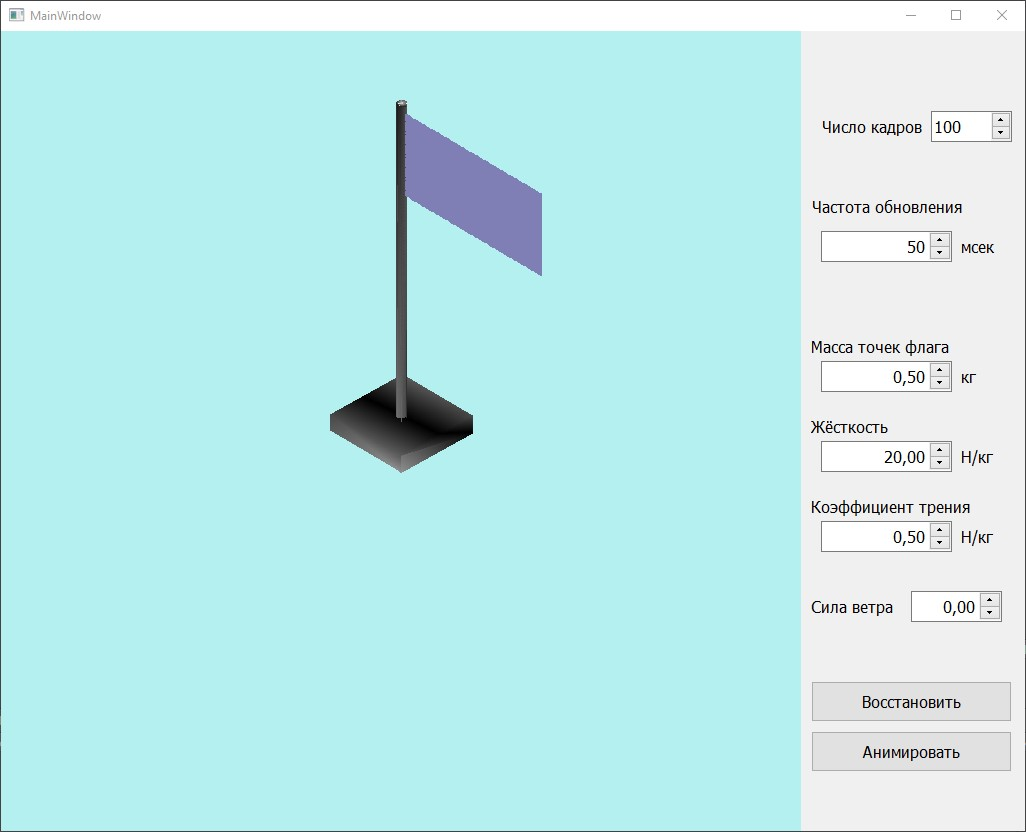
\includegraphics[scale=0.65]{gui.jpg}
	\caption{Окно программы}
	\label{fig:gui}
\end{figure}

\hspace{0.6cm} Окно состоит из двух частей: в левой части показывается результат рендеринга, в правой находится панель управления анимацией. В панель управления входят счётчики числа выполняемых кадров, частоты обновления, величины массы точек флага, величины жесткости, величины коэффициента трения, величины силы ветра, а также кнопки восстановления флага в изначальное состояние и запуска анимации.
Имеется возможность также осуществлять смещение, масштабирование и вращение объекта:
\begin{itemize}
	\item смещение осуществляется клавишами WASD;
	\item масштабирование осуществляется колесом мыши;
	\item вращение осуществляется движением мыши по "холсту" с зажатием правой кнопки мыши.
\end{itemize}

\section{Примеры работы}

\begin{figure}[ht!]
	\centering
	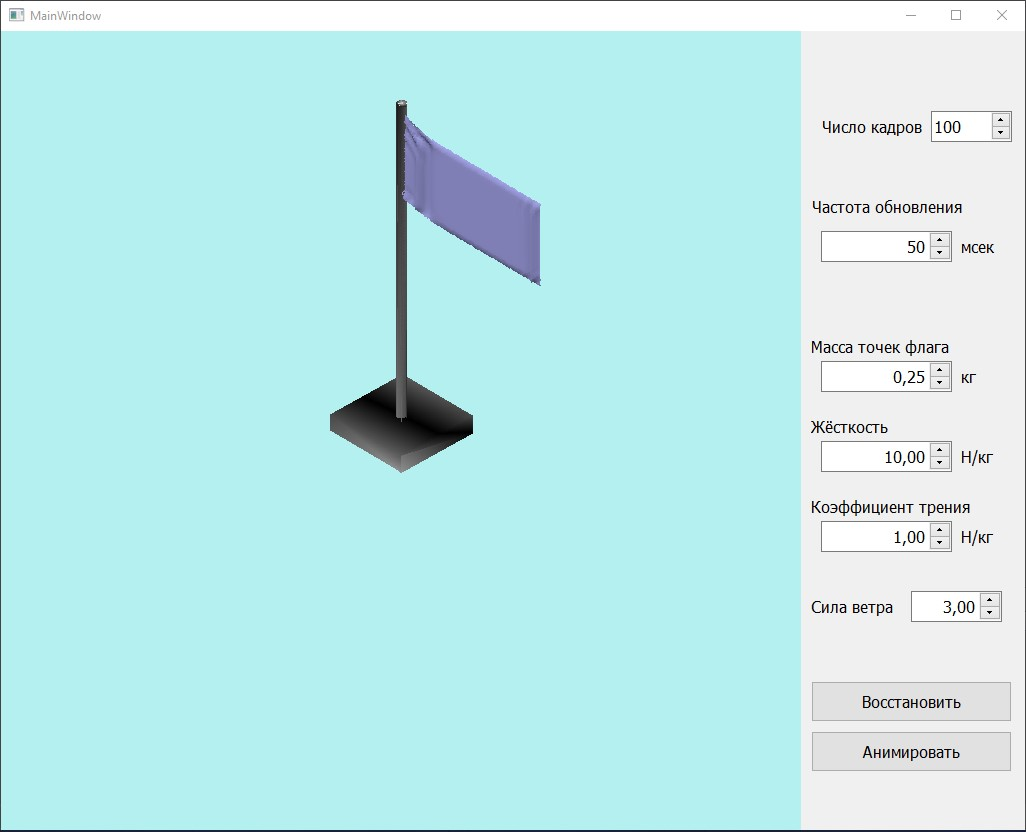
\includegraphics[scale=0.65]{example1.jpg}
	\caption{Пример результата первого запуска анимации}
	\label{fig:example}
\end{figure}

\begin{figure}[ht!]
	\centering
	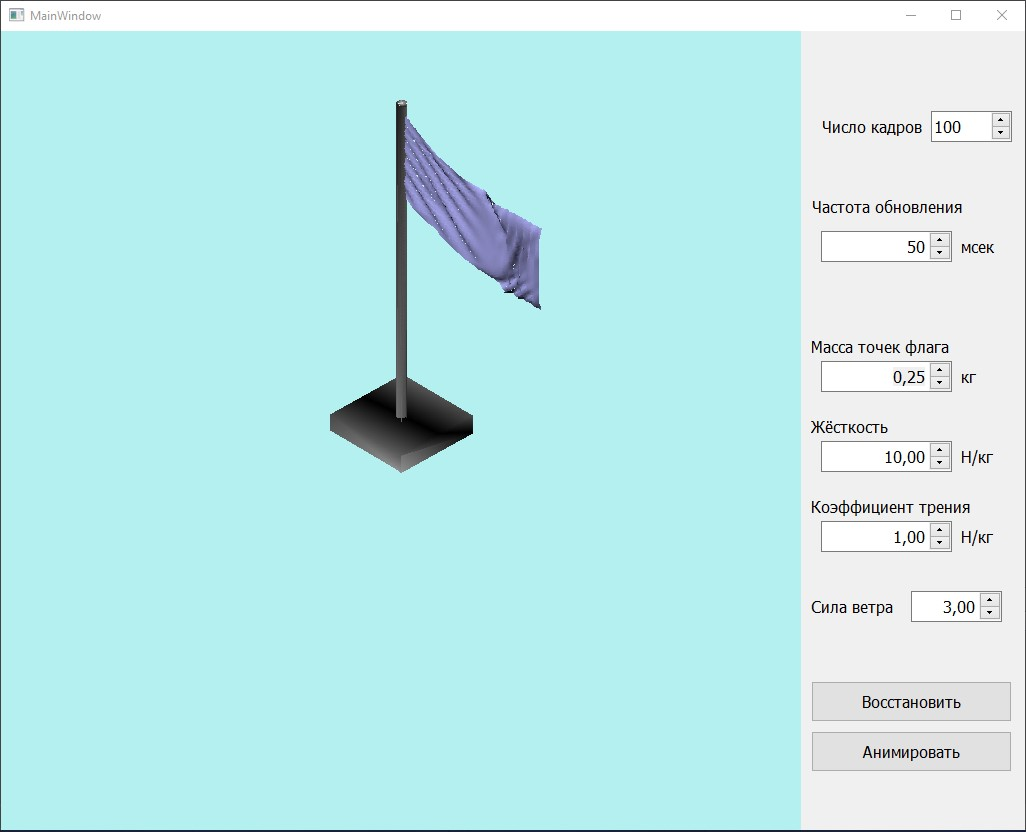
\includegraphics[scale=0.65]{example2.jpg}
	\caption{Пример результата анимации}
	\label{fig:example}
\end{figure}

\newpage

\section{Вывод}
\hspace{0.6cm}В данном разделе были рассмотрены требования к разрабатываемому программному обеспечению, средства реализации, использованные в процессе разработки, были приведены структуры данных, листинг кода к каждой из написанной структур данных. Было подробно расписано взаимодействие с интерфейсом и за что каждая часть интерфейса отвечает.
